% ==========================================================================
% Additional Task (K4): Perceptron Learning Algorithm for OR, NOT, AND Gates
%
% This is a standalone section meant to be pasted at the end of the main
% Experiment 1 report, right before the References section. It can also be
% compiled on its own with pdflatex, as long as the three figure PDFs below
% are in a figures/ folder next to this file.
% ==========================================================================

\section*{Additional Task: Perceptron Learning Algorithm for AND, OR, and NOT Gates (K4)}

A Single Layer Perceptron was coded from scratch in Python to learn the AND, OR, and NOT logic
gates. For each gate, the weights and bias were printed after every single weight update, and the
decision boundary was plotted after every update using only NumPy and Matplotlib.

\subsection*{Code}

\begin{verbatim}
"""
Additional Task: Perceptron Learning Algorithm for OR, NOT, and AND gates
Shows weights after every update and plots the decision boundary after
every weight update.
"""

import numpy as np
import matplotlib.pyplot as plt

# ----------------------------------------------------------------------
# Perceptron implementation with per-update logging
# ----------------------------------------------------------------------
class Perceptron:
    def __init__(self, n_inputs, learning_rate=0.1):
        self.weights = np.zeros(n_inputs)
        self.bias = 0.0
        self.lr = learning_rate
        self.history = []  # list of (weights copy, bias) after each update

    @staticmethod
    def step(z):
        return 1 if z >= 0 else 0

    def predict(self, x):
        z = np.dot(self.weights, x) + self.bias
        return self.step(z)

    def fit(self, X, y, epochs=10):
        # record the initial state before any update
        self.history.append((self.weights.copy(), self.bias))

        for epoch in range(1, epochs + 1):
            errors = 0
            for xi, target in zip(X, y):
                pred = self.predict(xi)
                error = target - pred
                if error != 0:
                    self.weights += self.lr * error * xi
                    self.bias += self.lr * error
                    errors += 1
                    self.history.append((self.weights.copy(), self.bias))
                    print(f"Epoch {epoch}, sample {xi}, target {target}, "
                          f"pred {pred} -> weights={self.weights}, bias={self.bias:.2f}")
            if errors == 0:
                print(f"Converged after epoch {epoch}, no errors left.\n")
                break
        return self.history


# ----------------------------------------------------------------------
# Plotting helper: decision boundary after each update
# ----------------------------------------------------------------------
def plot_decision_boundaries(X, y, history, gate_name, n_inputs):
    n_updates = len(history)
    n_cols = 4
    n_rows = int(np.ceil(n_updates / n_cols))

    fig, axes = plt.subplots(n_rows, n_cols, figsize=(4 * n_cols, 4 * n_rows))
    axes = np.array(axes).reshape(-1)

    for i, (w, b) in enumerate(history):
        ax = axes[i]

        if n_inputs == 2:
            # 2D input space, boundary is a line: w0*x0 + w1*x1 + b = 0
            for xi, target in zip(X, y):
                color = "seagreen" if target == 1 else "crimson"
                ax.scatter(xi[0], xi[1], c=color, s=100, edgecolor="black", zorder=3)

            x_vals = np.linspace(-0.5, 1.5, 100)
            if w[1] != 0:
                y_vals = -(w[0] * x_vals + b) / w[1]
                ax.plot(x_vals, y_vals, color="steelblue")
            elif w[0] != 0:
                x_boundary = -b / w[0]
                ax.axvline(x_boundary, color="steelblue")

            ax.set_xlim(-0.5, 1.5)
            ax.set_ylim(-0.5, 1.5)
            ax.set_xlabel("x1")
            ax.set_ylabel("x2")

        else:
            # 1D input space (NOT gate), boundary is a single point
            for xi, target in zip(X, y):
                color = "seagreen" if target == 1 else "crimson"
                ax.scatter(xi[0], 0, c=color, s=100, edgecolor="black", zorder=3)

            if w[0] != 0:
                x_boundary = -b / w[0]
                ax.axvline(x_boundary, color="steelblue")

            ax.set_xlim(-0.5, 1.5)
            ax.set_ylim(-1, 1)
            ax.set_xlabel("x1")
            ax.set_yticks([])

        title = "Initial" if i == 0 else f"Update {i}"
        ax.set_title(f"{title}\nw={np.round(w, 2)}, b={b:.2f}", fontsize=9)

    for j in range(n_updates, len(axes)):
        axes[j].axis("off")

    fig.suptitle(f"{gate_name} Gate: Decision Boundary After Each Weight Update", fontsize=13)
    plt.tight_layout()
    plt.savefig(f"{gate_name.lower()}_decision_boundaries.pdf", dpi=600)
    plt.show()


# ----------------------------------------------------------------------
# AND gate
# ----------------------------------------------------------------------
X_and = np.array([[0, 0], [0, 1], [1, 0], [1, 1]])
y_and = np.array([0, 0, 0, 1])

p_and = Perceptron(n_inputs=2, learning_rate=0.1)
history_and = p_and.fit(X_and, y_and, epochs=10)
plot_decision_boundaries(X_and, y_and, history_and, "AND", n_inputs=2)


# ----------------------------------------------------------------------
# OR gate
# ----------------------------------------------------------------------
X_or = np.array([[0, 0], [0, 1], [1, 0], [1, 1]])
y_or = np.array([0, 1, 1, 1])

p_or = Perceptron(n_inputs=2, learning_rate=0.1)
history_or = p_or.fit(X_or, y_or, epochs=10)
plot_decision_boundaries(X_or, y_or, history_or, "OR", n_inputs=2)


# ----------------------------------------------------------------------
# NOT gate
# ----------------------------------------------------------------------
X_not = np.array([[0], [1]])
y_not = np.array([1, 0])

p_not = Perceptron(n_inputs=1, learning_rate=0.1)
history_not = p_not.fit(X_not, y_not, epochs=10)
plot_decision_boundaries(X_not, y_not, history_not, "NOT", n_inputs=1)
\end{verbatim}

\subsection*{Training Log}

\textbf{AND gate:}
{\scriptsize
\begin{verbatim}
Epoch 1, sample [0 0], target 0, pred 1 -> weights=[0. 0.], bias=-0.10
Epoch 1, sample [1 1], target 1, pred 0 -> weights=[0.1 0.1], bias=0.00
Epoch 2, sample [0 0], target 0, pred 1 -> weights=[0.1 0.1], bias=-0.10
Epoch 2, sample [0 1], target 0, pred 1 -> weights=[0.1 0. ], bias=-0.20
Epoch 2, sample [1 1], target 1, pred 0 -> weights=[0.2 0.1], bias=-0.10
Epoch 3, sample [0 1], target 0, pred 1 -> weights=[0.2 0. ], bias=-0.20
Epoch 3, sample [1 0], target 0, pred 1 -> weights=[0.1 0. ], bias=-0.30
Epoch 3, sample [1 1], target 1, pred 0 -> weights=[0.2 0.1], bias=-0.20
Converged after epoch 4, no errors left.
\end{verbatim}
}

\textbf{OR gate:}
{\scriptsize
\begin{verbatim}
Epoch 1, sample [0 0], target 0, pred 1 -> weights=[0. 0.], bias=-0.10
Epoch 1, sample [0 1], target 1, pred 0 -> weights=[0.  0.1], bias=0.00
Epoch 2, sample [0 0], target 0, pred 1 -> weights=[0.  0.1], bias=-0.10
Epoch 2, sample [1 0], target 1, pred 0 -> weights=[0.1 0.1], bias=0.00
Epoch 3, sample [0 0], target 0, pred 1 -> weights=[0.1 0.1], bias=-0.10
Converged after epoch 4, no errors left.
\end{verbatim}
}

\textbf{NOT gate:}
{\scriptsize
\begin{verbatim}
Epoch 1, sample [1], target 0, pred 1 -> weights=[-0.1], bias=-0.10
Epoch 2, sample [0], target 1, pred 0 -> weights=[-0.1], bias=0.00
Converged after epoch 3, no errors left.
\end{verbatim}
}

\subsection*{Decision Boundary Plots}

\begin{figure}[h!]
\centering
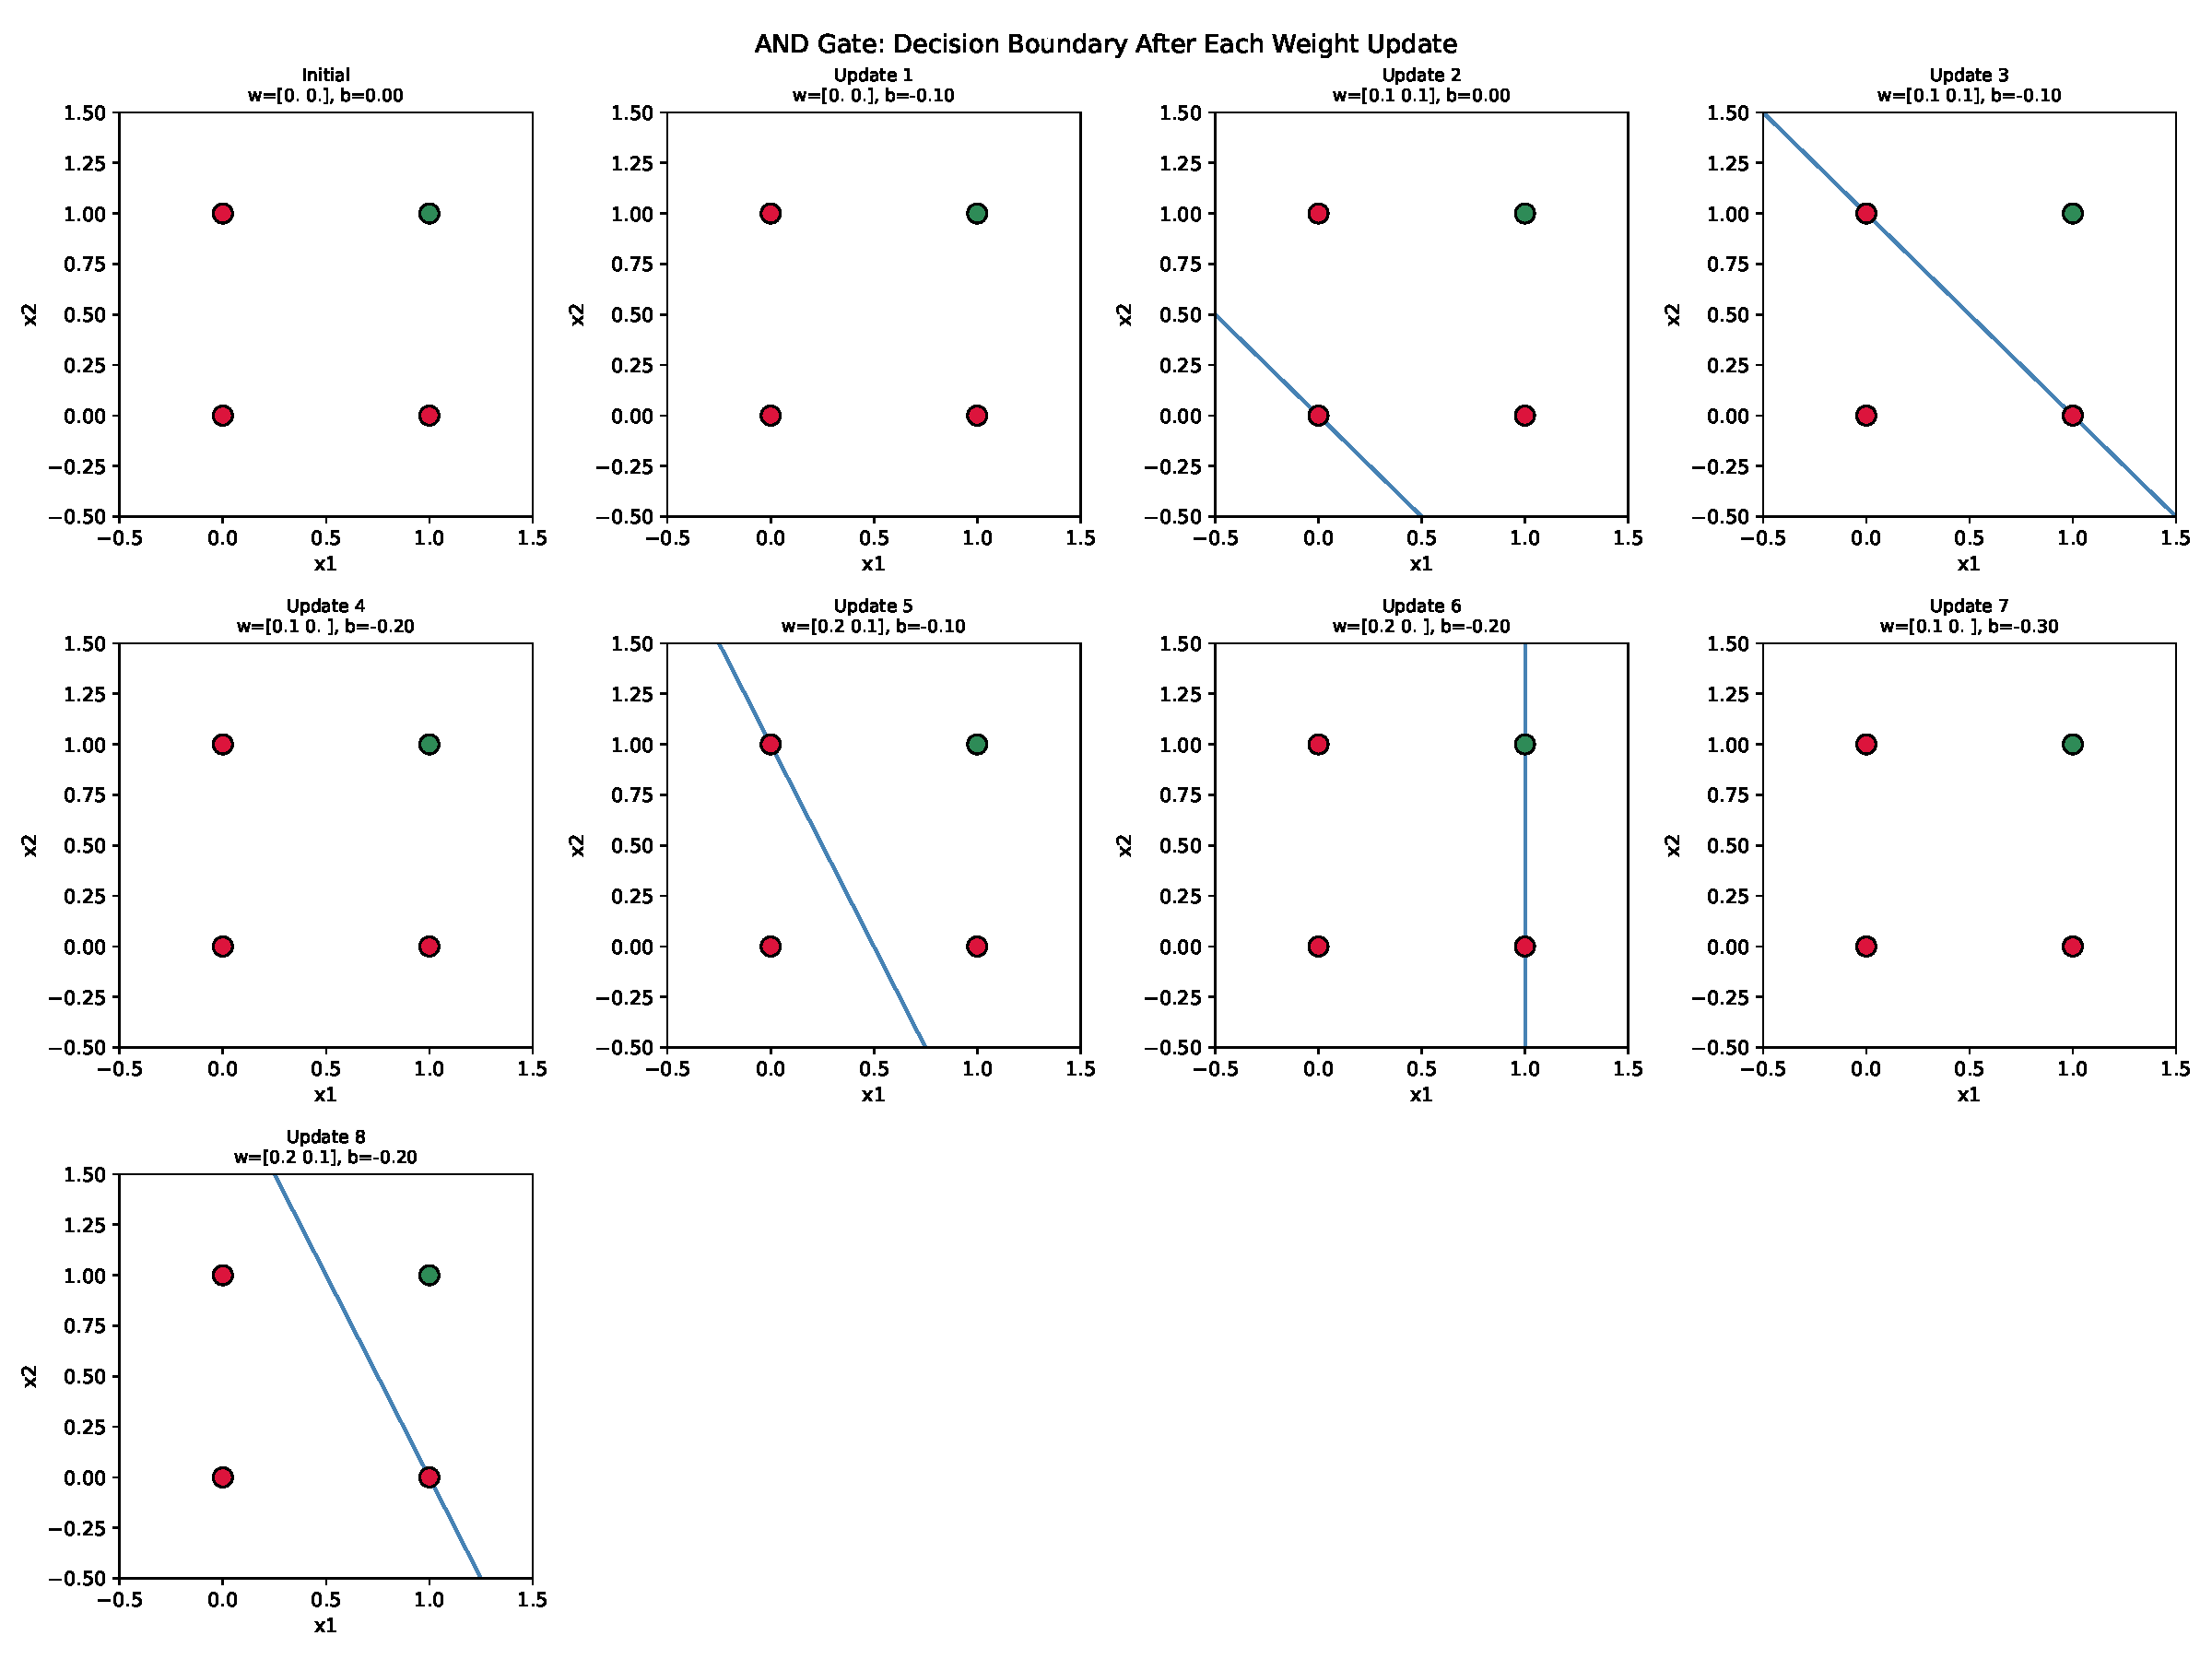
\includegraphics[width=0.95\textwidth]{and_decision_boundaries.pdf}
\caption{AND Gate: Decision Boundary After Each Weight Update.}
\end{figure}

\begin{figure}[h!]
\centering
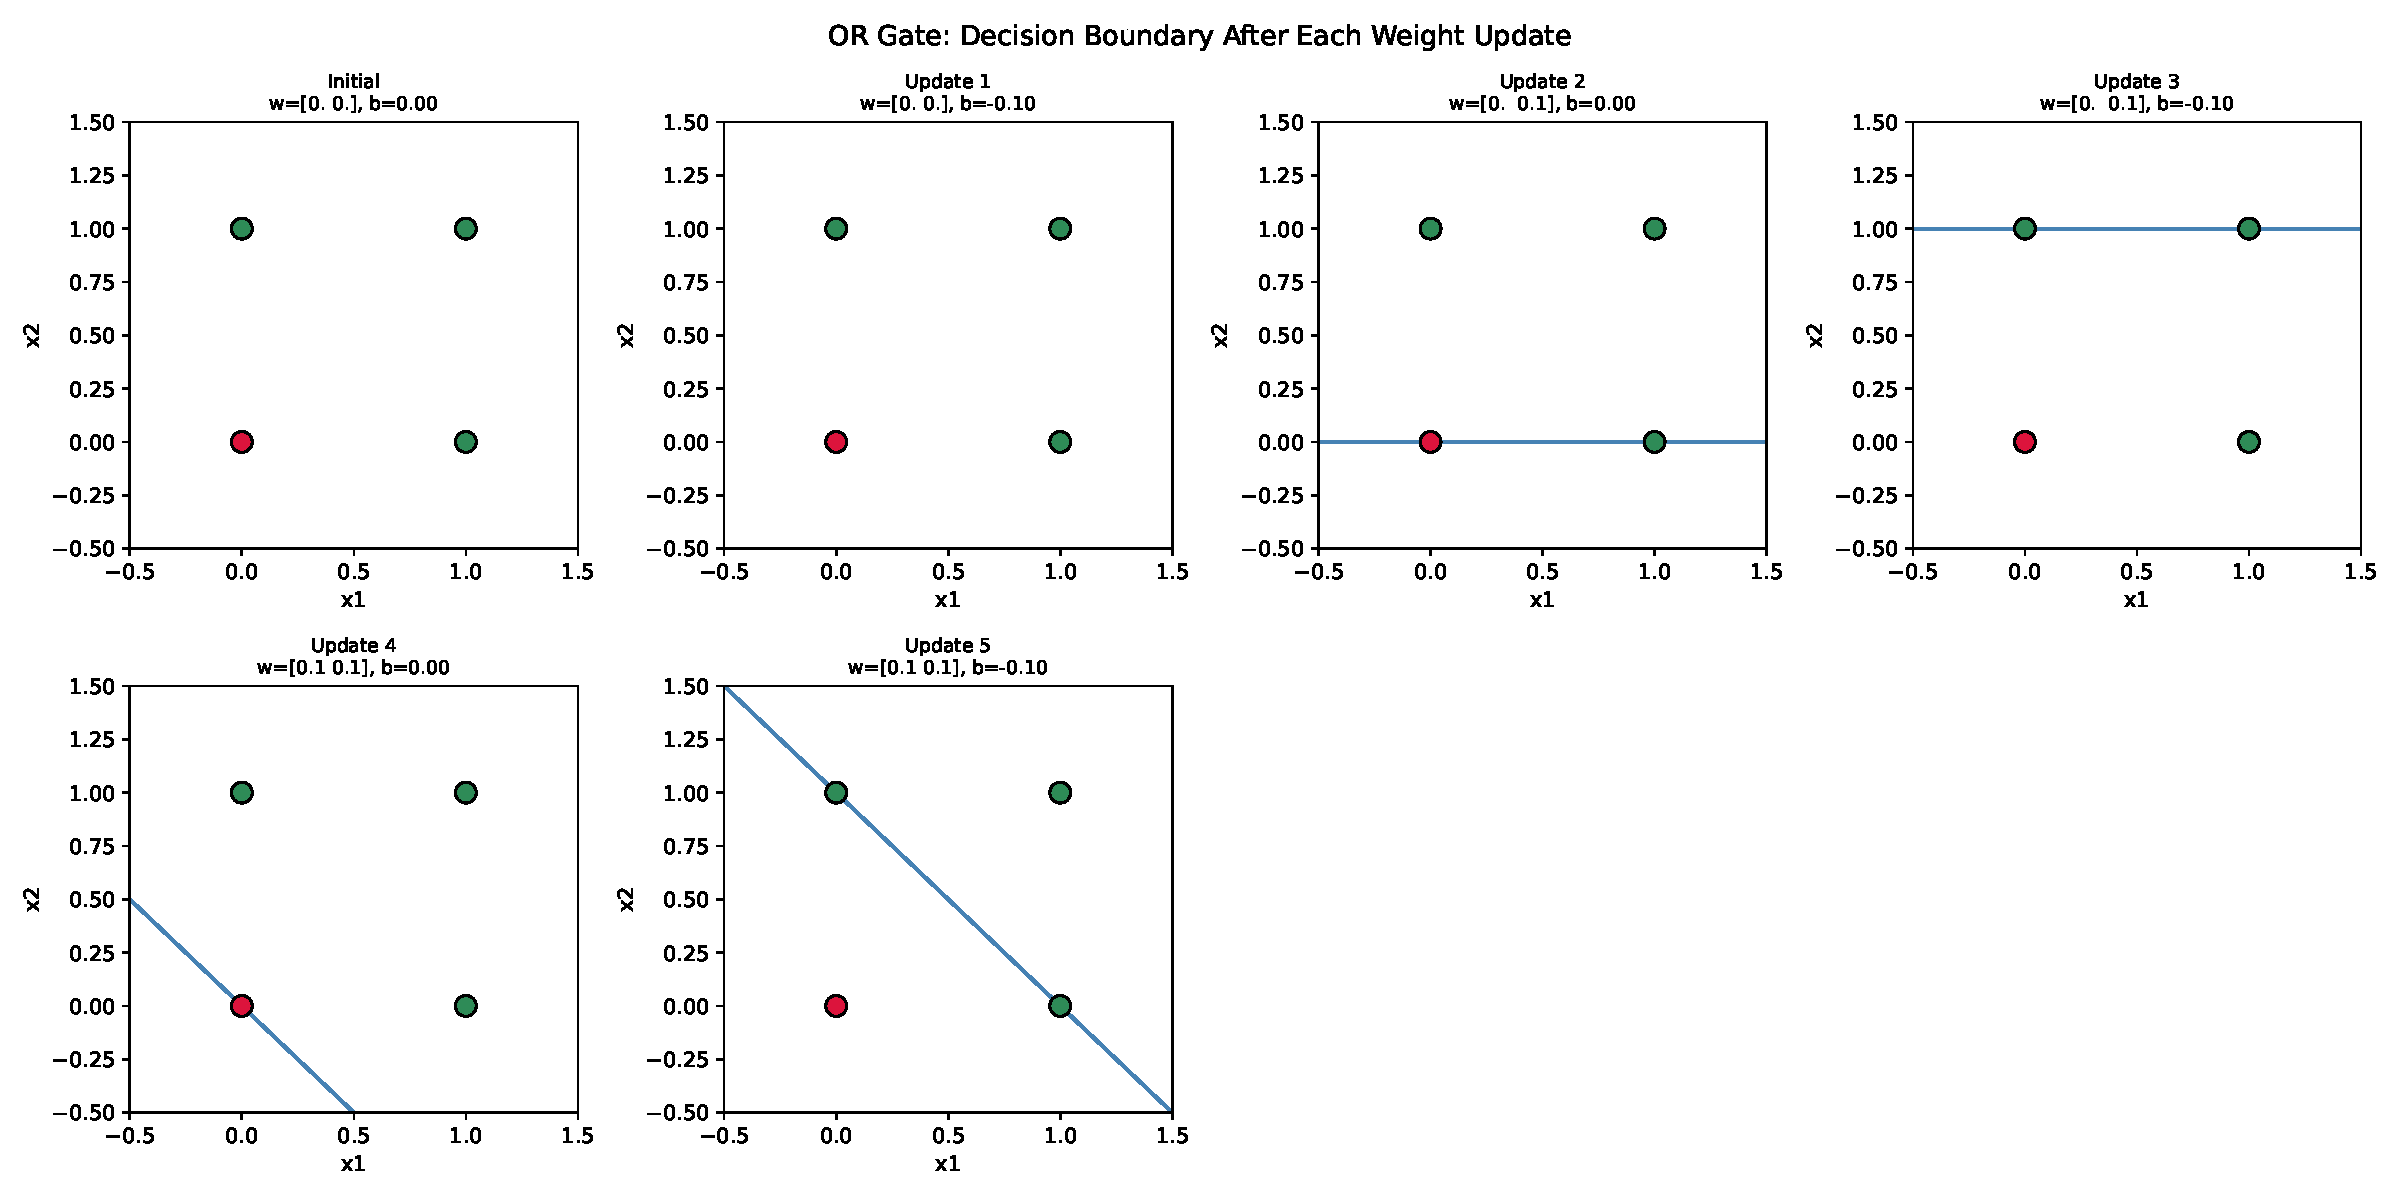
\includegraphics[width=0.95\textwidth]{or_decision_boundaries.pdf}
\caption{OR Gate: Decision Boundary After Each Weight Update.}
\end{figure}

\begin{figure}[h!]
\centering
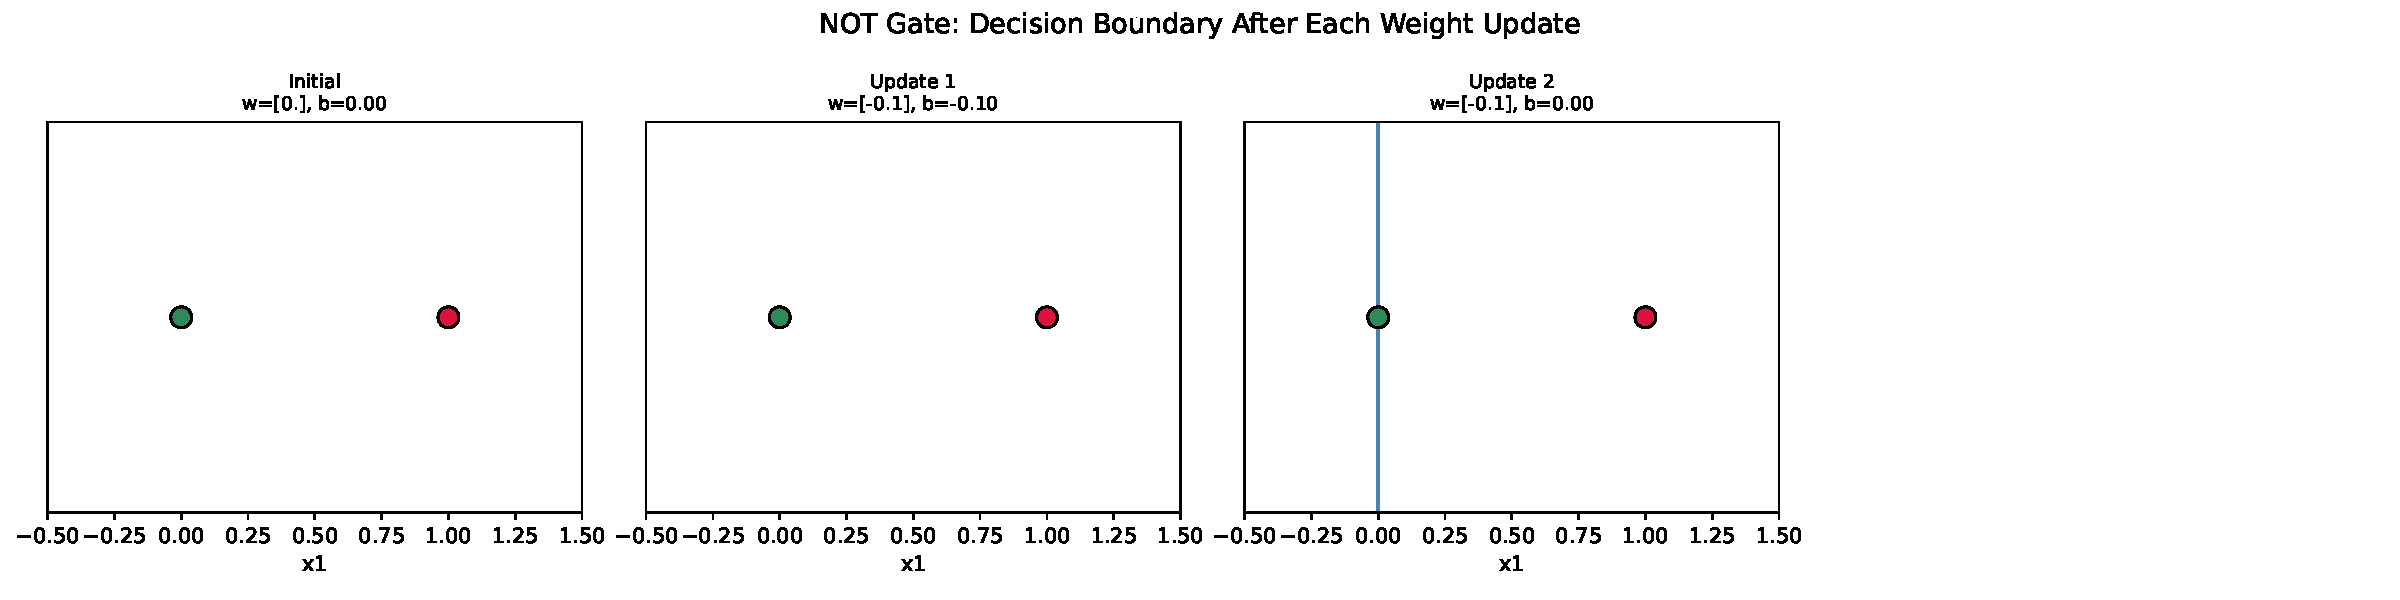
\includegraphics[width=0.95\textwidth]{not_decision_boundaries.pdf}
\caption{NOT Gate: Decision Boundary After Each Weight Update.}
\end{figure}

\noindent\textbf{Observation:} AND converges in 8 updates, OR in 5 updates, and NOT in 2 updates.
All three gates are linearly separable, so the perceptron finds a boundary that classifies every
sample correctly, unlike the XOR case discussed earlier in this report, which never converges.
